\documentclass[11pt]{article}
\usepackage{amsmath}
\usepackage[german]{babel}
\selectlanguage{german}
\usepackage[T1]{fontenc}
\usepackage[parfill]{parskip}
\usepackage{color}
\usepackage{xcolor}
\usepackage{tabto}
\usepackage{amsmath}
\usepackage{amssymb}
\usepackage{amsthm} %für das \qed Symbol. Außerdem gibt es eine proof environment
\usepackage{graphicx}
\usepackage{listings} % für code im Text
\usepackage{lstautogobble} % für Pseudo code wie im VL-Skript
%\usepackage[ruled,vlined,linesnumbered]{algorithm2e}
\usepackage[ruled,noend,noline,nofillcomment,linesnumbered]{algorithm2e}
\DontPrintSemicolon

\SetKw{KwBy}{by}

\usepackage{tikz}
\usepackage[utf8]{inputenc}
%\usepackage{algpseudocode}
\newcommand{\LD}{\langle}
\newcommand{\RD}{\rangle}
 \usepackage[utf8]{inputenc}
\usepackage{geometry} %to change the site margin
\usepackage[justification=centering]{caption}
\geometry{left=3cm, right=2cm, top=2cm, bottom=2cm}
\theoremstyle{remark}
\newtheorem*{Behauptung}{Behauptung}
\renewcommand\thesection{Aufgabe \arabic{section}}
\renewcommand\thesubsection{\alph{subsection})}
\usepackage{mathtools}
\DeclarePairedDelimiter\ceil{\lceil}{\rceil}
\usepackage{array}   % for \newcolumntype macro
\newcolumntype{C}{>{$}c<{$}} % math-mode version of "l" column type
\newcommand\inductioneq{\stackrel{\mathclap{\normalfont\mbox{I.B.}}}{=}}
\newcommand*{\CommentInLine}{\tcc*[f]}
\def\checkmark{\tikz\fill[scale=0.4](0,.35) -- (.25,0) -- (1,.7) -- (.25,.15) -- cycle;} 


\title{Übung 3: Algorithmen und Datenstrukturen}
\author{
\begin{tabular}{|r|c|c|c|c|c|c|}\hline
   Theodor Bajusz  & 7159556 & x& x& x& x& \phantom{0} \\ \hline
    Valerij Dobler & 7068135 & x& x& x& x&  \\ \hline
    Matz Radloff & 6946325 & x& x& x& x&  \\ \hline
    Robin Wannags & 6948409 & x& x& x& x& \\\hline
\end{tabular}
}

\begin{document}
\maketitle

\section{}
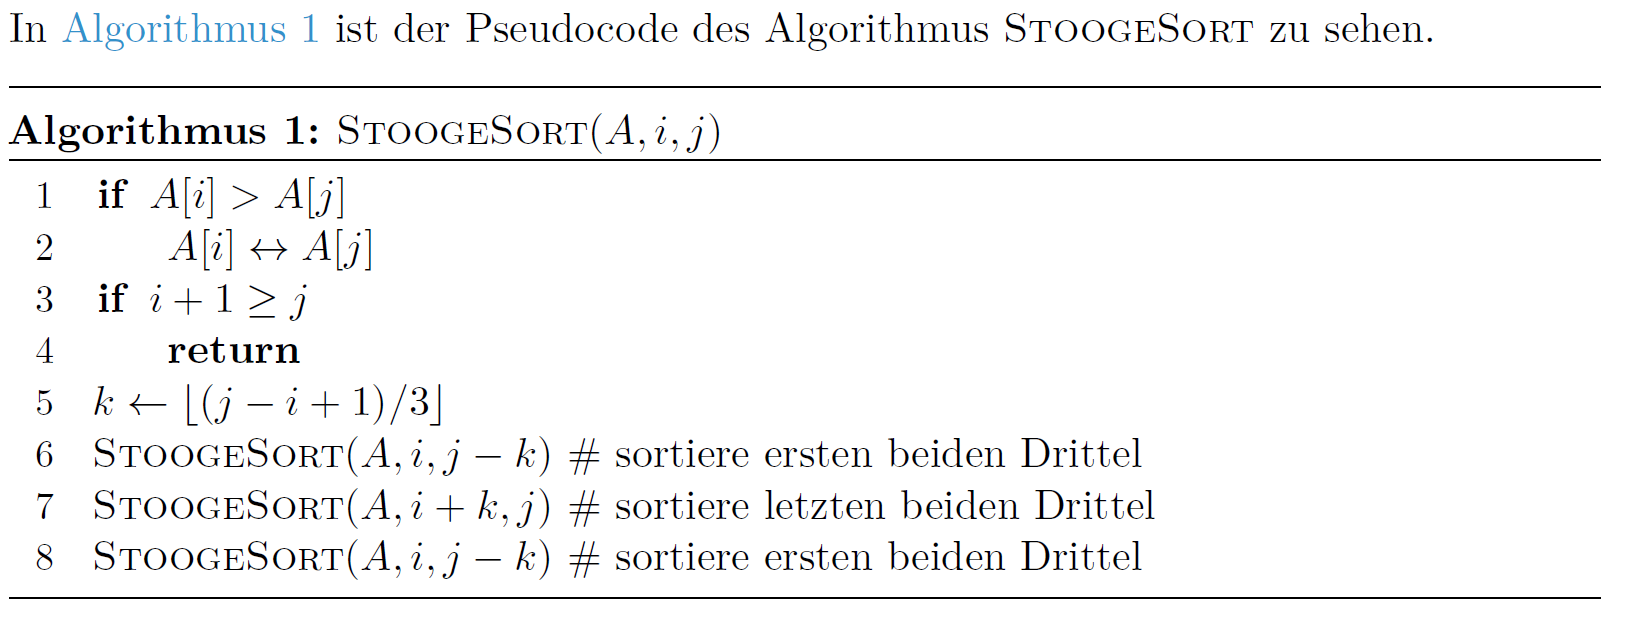
\includegraphics[width=\linewidth]{Stoogesort_Pseudocode.PNG}
\subsection{}
Beweisen Sie die Korrektheit von $STOOGESORT$. Das heißt, beweisen Sie dass der Aufruf StoogeSort(A, 1, length(A)) das Array A korrekt sortiert. Führen Sie dazu einen Induktionsbeweis über die Länge von A. (5 Punkte)

Induktionsbehauptung:
StoogeSort(A, 1, length(A)) sortiert das Array A korrekt.


Induktionsbeginn:

Zeile 3 und 4 stellen sicher, dass der Algorithmus bei Arrays mit der Länge 1 und 2 abbricht.

Arrayintervalle der Länge 1 sind trivialerweise sortiert. Für Intervalle der Länge 2 werden, falls sie falsch sortiert sind durch die Abfrage in Zeile 1 immer in die richtige Reihenfolge gebracht.
//

Induktionsschritt:

Für Intervalle größer als 2 wird in k ein Index bestimmt, welcher annähernd ein Drittel des Intervalls markiert. Mit Hilfe von k wird StoogeSort auf den ersten beiden Dritteln aufgerufen. Ziel dabei ist, dass Elemente, welche im dritten Drittel sein müssen, ins zweite Drittel "geschoben" werden. Danach geschieht ein Aufruf an StoogeSort mit den letzten beiden Dritteln. Dabei werden Elemente, welche im ersten Drittel sein müssen, ins zweite Drittel "geschoben". Das dritte Drittel hat dann nur Elemente, welche auch dort sein müssen. Beim letzten Aufruf an StoogeSort werden wieder die ersten beiden Drittel erneut sortiert. Dabei werden endgültig die Elemente, die im ersten Drittel sein müssen, auch ins erste Drittel "geschoben".

%<3,1,2> => <2,1,3> => <1,2,3>

%<4,3,2,1> => <1,3,2, 4> => <1,2,3,4>
Daraus folgt, dass Arrays mit der Länge A immer korrekt sortiert sind.


\subsection{}
Analysieren Sie die worst-case Laufzeit von StoogeSort im $O$-Kalkül. Nutzen Sie
dazu eine geeignete Rekursionsgleichung. (4 Punkte)\\

$n = length(A)$ \\

\[
T(n) := \left\{
    \begin{array}{ll}
        O(1), &  \textrm{für} \; n < 3 \\
        3 \cdot T(\lfloor n\cdot 2/3 \rfloor),  & \, \textrm{sonst} \\
    \end{array}
    \right.
\]

Rechnung:
$\begin{tabular}{ll}
    &\geq 3 \cdot T(n \cdot 2 / 3) \\
    &\geq 3 \cdot (3 \cdot T(n \cdot (2/3)^2)) \\
    &\geq 3 \cdot (3 \cdot (3 \cdot T(n \cdot (2/3)^3))) \\
    & \qquad \qquad \quad \vdots \\
\end{tabular}$

Wir berechnen wie oft Rekursionsaufrufe stattfinden, bis die Abbruchbedingung $n<3$ erreicht ist:
$$3 < n \cdot (2/3)^k$$
$$3 \cdot (3/2)^k < n$$
$$log_{1,5}3 + k < log{1,5}n$$
$$k < log_{1,5}n - log_{1,5}3$$
$$k < log_{1,5}(\frac{n}{3})$$
$$k < \frac{log(\frac{n}{3})}{log(1,5)}$$

Wenn wir nun Ganzzahlige k suchen, welche diese Ungleichung genügen, müssen wir das Ergebnis aufrunden:

$$k < \lceil \frac{log(\frac{n}{3})}{log(1,5)} \rceil$$.

$T(n)$ wird $n^{log_{1,5}(\frac{n}{3})}$-mal ausgeführt, bevor der Rekursionsabbruch stattfindet. Daraus folgt, dass $T(n) = O(n^{log_{1,5}(\frac{n}{3})})$

\section{}
\subsection{}
Sortieren Sie das Array $A = \langle20, 13, 8, 5, 2, 12, 9\rangle$ mithilfe des $QuickSort$-Algorithmus
aus der Vorlesung. Stellen Sie den Inhalt des Arrays nach jedem Aufruf von
$Partition$ dar. (3 Punkte)\\

\begin{center}
    \begin{tabular}{|r|c|} \hline
        Durchlauf $n$ & Array $A$ \\ \hline
        0 & $\langle 20, 13, 8, 5, 2, 12, 9 \rangle$\\ \hline
        1 & $\langle 8, 5, 2, \bold{9}, 20, 12, 13 \rangle$\\ \hline
        2 & $\langle \bold{2}, 5, 8, \bold{9}, 20, 12, 13 \rangle$\\ \hline
        3 & $\langle \bold{2}, \bold{5}, \bold{8}, \bold{9}, 20, 12, 13 \rangle$\\ \hline
        4 & $\langle \bold{2}, \bold{5}, \bold{8}, \bold{9}, \bold{12}, \bold{13}, \bold{20} \rangle$\\ \hline
    \end{tabular}
\end{center}

\subsection{}
Welchen Einfluss auf die Laufzeit hat allgemein die Auswahl des Pivotelements bei
$QuickSort$? Skizzieren Sie worst-case- und best-case-Eingaben für eine konkrete
Auswahl des Pivotelements (z.B. immer am linken oder rechten Rand). Begründen
Sie Ihre Antwort. (2 Punkte)\\

Die Wahl des Pivotelements entscheidet beim nächsten Rekursionsaufruf über die Größe der beiden Intervalle. Falls das Pivotelement das kleinste oder größte Element im Intervall der Länge $n$ des Arrays ist, dann wird ein Quicksort-Aufruf mit einem Intervall Länge n-1 aufgerufen und das andere mit der Länge 1.

Betrachten wir eine Folge $a=a_1, a_2, a_3, \ldots, a_n$, wobei $\exists i\exists j \in \mathrm{N}_\leqn$ und $i \neq j$


\subsection{}
Ein Sortieralgorithmus ist stabil, wenn er die Reihenfolge der Arrayeinträge mit gleichem Wert bewahrt.
Ist der $QuickSort$-Algorithmus aus der Vorlesung stabil? Begründen Sie Ihre
Antwort. (2 Punkte)\\

Der Sortier-Algorithmus ist nicht stabil was mit folgendem Beispiel einfach zu widerlegen ist: \\
1 ist das Pivotelement 
$\{2_1, 2_2, 1\}$ $\xrightarrow{QuickSort}$ $\{1, 2_2, 2_1\}$\\

Anfangs wird der das $l$ auf den Index $2_1$ gesetzt. Unser $r$ ist dabei auf den Index 1 gesetzt. Das $i$ wird auf den Index $l-1$ gesetzt, also einen Platz links vom Index $l$. Außerdem wird nun $j$ auch auf den Index $2_1$ gesetzt. Das $j$ wandert nun einen Index nach rechts und zeigt auf $2_2$. Nun werden die Positionen von den Indizes $2_1$ und $2_2$ im Array vertauscht, da die Bedingung $if A[j] \leq x$ gilt. Nun rückt das $i$ einen Index weiter nach rechts. Da das $j$ im nächsten Schritt auf den Index $1$ zeigt und die Bedingung $if A[j] \leq x$ wieder gilt, wird Index $1$ die Stelle mit dem Index $2_1$ tauschen. Nun erhalten wir die sortierte, aber nicht stabile Reihenfolge $1, 2_2, 2_1$. Würde die Bedingung einzeln die Relation kleiner und einzeln die Relation gleich prüfen, dann könnte man eine stabile Sortierung mit $QuickSort$ erhalten.

\newpage

\section{}
\subsection{}
Beschreiben Sie einen Algorithmus in Pseudocode, der zwei vollständige Max-Heaps gleicher Größe $n$ vereinigt. Gehen Sie dazu davon aus, dass die Heaps keine gemeinsamen Elemente enthalten. (2 Punkte)

\begin{algorithm}
\caption{TwoMaxHeap(A1, A2)}
    $A \gets Array[2n] \quad$ \CommentInLine{Neues Array der Größe 2n} \\
    $k \gets 1$ \\
    \For{$i \gets 1$; $i \leq length(A1)$$; $i \gets i + 1$} { 
        $A[k] \gets A1[i]$ \\
        $k \gets k + 1$\\
    }
    \For{i \gets 1; i \leq length(A2); i \gets i + 1} {
        $A[k] \gets A2[i]$ \\
        $k \gets k + 1$\\
    }
    \CommentInLine{Sortiere das Array aufsteigend mithilfe von Countingsort in linearer Zeit} \\
    countingsort(A) \\
    \CommentInLine{Sortierungsreihenfolge umkehren}\\
    \For{i \gets 1; i \leq \lfloor length(A)/2\rfloor; i \gets i + 1}{
        $A[i]\leftrightarrow A[length(A)-i]$
    }
\end{algorithm}

Durch unseren Algorithmus entsteht ein sortiertes Arrays was widerrum ein ein Heap ist.

\subsection{}
Analysieren Sie die Laufzeit ihres Algorithmus. (2 Bonuspunkte, wenn sie beweisen
können, dass ihr Algorithmus in $O(n)$ läuft.) (2 Punkte)\\

\begin{tabular}{|c|c|} \hline
    Zeile & Laufzeit \\ \hline
    $1$ & $O(1)$ \\  \hline
    $2$ & $O(1)$ \\ \hline
    $3$ & $O(n)$ \\ \hline
    $4$ & $O(1)$ \\ \hline
    $5$ & $O(2)$\\ \hline
    $6$ & $O(n)$ \\ \hline
    $7$ & $O(1)$ \\ \hline
    $8$ & $O(2)$ \\ \hline
    $9$ & $O(2n)$ \\ \hline
    $10$ & $O(n)$ \\ \hline
    $11$ & $O(2)$ \\ \hline
\end{tabular}

\[
O(1) + O(1) + O(n) \cdot (O(1) + O(2)) + O(n) \cdot (O(1) + O(2)) + O(2n) + O(n) \cdot O(2) = O(5n) = O(n)
\]

Für die Bonuspunkte: Wir können hier $CountingSort$ anwenden, weil wir davon ausgehen konnten, dass beide Heaps keine gemeinsamen Elemente beinhalten, und dass wir wissen, dass der Wertebereich durch die größere Zahl der beiden Maxima ($max\{A1[1], A2[1]\}$ beschränkt ist. Wobei $max$ die Mathematische Maximum-funktion ist:
$$max\{a,b\} = \begin{cases}
a & a \geq b \\
b & \, \text{sonst}
\end{cases}$$
Und $A1\left[1\right] := max(A1)$ und $A2\left[1\right] := max(A2)$ jeweils die größten Elemente beider Heaps $A1$ und $A2$ sind.

 in O(n²)
 \begin{algorithm}
 \caption{TwoMaxHeapNonLinear(A1, A2)}
     $A \gets Array[2n] \quad $\CommentInLine{Neues Array der Größe $2n$} \\
     \While{length(A1) > 0 || length(A2) > 0}{
         \If{length(A1) == 0 || max(A1) < max(A2)} {
             insert(A, deleteMax(A2)) \\
         }
         \Else {
             insert(A, deleteMax(A1)) \\
         }
     }
 \end{algorithm}

\end{document}